\chapter{Introduction to Logic}

The word \emph{logic} is used in two senses:
\begin{itemize}
    \item A set of principles that underlie the organization of elements within a system (e.g., a computer program, an electronic device, a communication protocol)
    \item Reasoning conducted according to strict rules that preserve validity
\end{itemize}
In computer science, these two meanings converge: first, we formally describe the given system, and then we \emph{formally reason} about it (in practical applications, this is done automatically), i.e., we derive valid \emph{inferences} about the system using some \emph{(formal) proof system}.

Practical applications of logic in computer science include software verification, logic programming, SAT solving, automated reasoning, database theory, knowledge-based representation, and many others. Moreover, logic (to a greater extent than mathematics) is a fundamental tool for describing theoretical computer science.


\section{Propositional Logic}

Now let's demonstrate logic in action with two real-life examples (from the lives of a treasure hunter and a theoretical computer scientist):


\subsection{Example: Treasure Hunting}

\begin{tcolorbox}
\begin{example}
While searching for treasure in a dragon's lair, we encountered a fork in the path with two corridors. We know that at the end of each corridor, there is either treasure or a dragon, but not both. A dwarf we met at the fork told us, ``At least one of these two corridors leads to the treasure,'' and after some further urging (and a small bribe), she also said, ``The first corridor leads to a dragon.'' It is well known that dwarves you meet in a dragon's lair either always tell the truth or always lie. Which way should we go?
\end{example}
\end{tcolorbox}


\subsection{Formalization in Propositional Logic}

We will begin by formalizing the situation and our knowledge in propositional logic. A \emph{proposition} is a statement to which we can assign a truth value: \emph{True} (1) or \emph{False} (0). Some propositions can be expressed using simpler propositions and logical connectives, e.g., ``(The dwarf is lying) \emph{if and only if} (the second corridor leads to a dragon)'' or ``(The first corridor leads to treasure) \emph{or} (the first corridor leads to a dragon).'' If a proposition cannot be decomposed in this way, it is called a \emph{simple proposition}, \emph{atomic proposition}, or \emph{propositional variable}.

Thus, we will describe the entire situation using \emph{propositional variables}. We can also think of these as simple yes/no questions we need to answer to know everything about the given situation. Let's choose ``The treasure is in the first corridor'' (denote as \(p_1\)), and ``The treasure is in the second corridor'' (\(p_2\)). Other propositional variables could be considered, such as ``There is a dragon in the first corridor'' (\(d_1\)) or ``The dwarf is telling the truth'' (\(t\)). However, these can be expressed using \(\{p_1, p_2\}\), e.g., \(t\) holds if and only if \(p_1\) does not hold. That is, if we know the truth values of \(p_1, p_2\), the truth values of \(d_1, t\) are uniquely determined. A smaller number of propositional variables means a smaller search space.

Next, we will express all our knowledge as (\emph{compound}) propositions and write them in formal notation in the \emph{language} of propositional logic over the set of atomic propositions \( \mathbb{P} = \{p_1, p_2\} \), using symbols representing logical connectives: \( \neg \) (``not X'', \emph{negation}), \( \land \) (``X and Y'', \emph{conjunction}), \( \lor \) (``X or Y'', \emph{disjunction}), \( \limplies \) (``if X, then Y'', \emph{implication}), \( \liff \) (``X if and only if Y'', \emph{equivalence}), and parentheses (, ). It is worth mentioning that disjunction is not exclusive; that is, ``X or Y'' holds even if both X and Y hold, and implication is purely logical: ``if X, then Y'' holds whenever X does not hold or Y holds.

The information that the corridor contains either a treasure or a dragon, but not both, is already encoded in our choice of propositional variables: the presence of a dragon is the same as the absence of treasure. The dwarf's statement that ``The first corridor leads to a dragon'' is thus expressed as ``It is not the case that the treasure is in the first corridor,'' formally \(\neg p_1\). The statement that ``At least one of these two corridors leads to the treasure'' is expressed as ``The treasure is in the first corridor or the treasure is in the second corridor,'' formally \( p_1 \lor p_2\). The information that dwarves either always tell the truth or always lie can be understood to mean that either both our propositions hold or the negations of both our propositions hold, formally:
\[
    (\neg p_1 \land (p_1 \lor p_2)) \lor (\neg (\neg p_1) \land \neg (p_1 \lor p_2))
\]
Let us denote this proposition as \( \varphi \) (from the word ``formula''; propositions are sometimes also called \emph{propositional formulas}). In our example, all information can be expressed with a single proposition. But in practice, we often need more propositions, sometimes even infinitely many (for example, if we want to describe the execution of a computer program and we do not know in advance how many steps it will take). We then describe the situation using a set of propositions, called a \emph{theory}, here \( T = \{ \varphi \} \). The propositions in \( T \) are also called \emph{axioms} of the theory~\( T \)\footnote{Terminology in logic often comes from its application in mathematics.}.


\subsection{Models and Consequences}

Is our information sufficient to determine whether there is treasure in one particular corridor? In other words, we are asking if one of the propositions \( p_1 \) or \( p_2 \) is a logical \emph{consequence} of the proposition \( \varphi \) (or the theory \( T \)). What does this mean?

Let's imagine that there are several ``worlds'' differing in what is at the end of the first and second corridors. For example, in one of the worlds, there is treasure at the end of the first corridor and a dragon at the end of the second corridor. We can describe this world using a truth valuation of the propositional variables: \( p_1 = 1, p_2 = 0 \). Such a valuation is called a \emph{model} of the language \( \mathbb{P} = \{p_1, p_2\} \) and we write it succinctly as \( v = (1,0) \) (\(v\) from the word ``valuation''). Thus, we have a total of four different worlds, described by the \emph{models of the language}:
\[
    \M_\mathbb{P} = \{(0,0), (0,1), (1,0), (1,1)\}.
\]

Is the world described by the model \( v = (1,0) \) consistent with the information we have, i.e., does the proposition \( \varphi \) (or the theory \( T \)) \emph{hold} in it? We can easily determine the truth value of the (compound) proposition \( \varphi \) in the model \(v\), denote it \( v(\varphi) \): We know that \( v(p_1) = 1 \) and \( v(p_2) = 0 \), so \( v(\neg p_1) = 0 \), and also \( v(\neg p_1 \land (p_1 \lor p_2)) = 0 \) (it is a conjunction of two propositions, and the first conjunct is false in the model \( v \)). Similarly, \( v(p_1 \lor p_2) = 1 \) (because \( v(p_1) = 1 \)), so \( v(\neg(p_1 \lor p_2)) = 0 \), and \( v(\neg (\neg p_1) \land \neg (p_1 \lor p_2)) = 0 \). The proposition \( \varphi \) is a disjunction of two propositions, neither of which holds in the model \(v\), so \( v(\varphi) = 0 \).

A keen reader will surely see the tree structure of the proposition \( \varphi \) and the step-by-step evaluation of \( v(\varphi) \) from the leaves to the root. We will present a formal definition in the next chapter.

Similarly, we determine the truth values of the proposition \( \varphi \) in other models. We find that the set of \emph{models of the proposition} \( \varphi \) (or the \emph{models of the theory} \( T \)), i.e., the set of all models of the language in which \( \varphi \) (or all axioms of the theory \( T \)) holds, is
\[
    \M_\mathbb{P}(\varphi) = \M_\mathbb{P}(T) = \{(0,1)\}.
\]
We see that our information uniquely determines the model \( (0,1) \), the world in which there is a dragon in the first corridor and treasure in the second corridor. In general, there can be more models; we only need to know that in every model of \( \varphi \) (or of \(T \)) the proposition \( p_2 \) holds, to conclude that \( p_2 \) is a \emph{consequence} of the theory \( T \); we also say that \( p_2 \) \emph{holds} in the theory \( T \).


\subsection{Proof Systems}

The approach we have chosen is very inefficient. If we have \( n \) propositional variables\footnote{In practice, we commonly have thousands of variables.}, there are \( 2^n \) models of the language, and it is practically impossible to check the validity of the theory in each of them. This is where \emph{proof systems} come into play. In a given proof system, a \emph{proof} of a proposition \( \psi \) from a theory \( T \) is a precisely, formally defined syntactic object that includes an easily (mechanically) verifiable ``proof'' (reason) that \( \psi \) holds in \( T \), and which can be searched for (using a computer) purely based on the structure of the proposition \( \psi \) and the axioms of the theory \( T \) (``syntax''), i.e., without having to deal with models (``semantics'').

We want two properties from a proof system:
\begin{itemize}
    \item \emph{soundness}, i.e., if we have a proof of \( \psi \) from \( T \), then \( \psi \) holds in \( T \), and
    \item \emph{completeness}, i.e., if \( \psi \) holds in \( T \), then there exists a proof of \( \psi \) from \( T \),
\end{itemize}
where soundness is a necessity (without it, searching for proofs makes no sense), and completeness is a desirable property, but an efficient proof system can be useful even if not everything that holds can be proven.

Here we briefly outline two proof systems: the \emph{method of analytic tableaux} and the \emph{resolution method}. They will be formally introduced later, and we will prove soundness and completeness for both of them. Both of these proof systems are based on \emph{proof by contradiction}, i.e., they assume the validity of the axioms from \( T \) and the negation of the proposition \( \psi \), and try to reach a contradiction.


% todo


\subsection{Tableau Method}

In the method of analytic tableaux, a proof is a \emph{tableau}: a tree whose nodes are labeled with assumptions about the validity of propositions. Let's look at an example of a tableau in Figure~\ref{figure:tableaux-proof-example}.

\begin{figure}
    \centering
    \begin{forest}
    [False \( p_2 \)
        [True \( (\neg p_1 \land (p_1 \lor p_2)) \lor (\neg (\neg p_1) \land \neg (p_1 \lor p_2)) \) 
            [True \( \neg p_1 \land (p_1 \lor p_2) \)
                [True \( \neg p_1 \)
                    [True \( p_1 \lor p_2 \)
                        [False \( p_1 \)
                            [True \( p_1 \), tikz={\node[fit to=tree,label=below:\emph{fail}] {};}
                            ]
                            [True \( p_2 \), tikz={\node[fit to=tree,label=below:\emph{fail}] {};}
                            ]
                        ]
                    ]
                ]
            ]
            [True \( \neg (\neg p_1) \land \neg (p_1 \lor p_2) \)
                [True \( \neg (\neg p_1) \)
                    [True \(\neg (p_1 \lor p_2) \)
                        [False \( (\neg p_1) \)
                            [True \( p_1 \)
                                [False \(p_1 \lor p_2 \)
                                    [False \(p_1\)
                                        [False \(p_2\), tikz={\node[fit to=tree,label=below:\emph{fail}] {};}
                                        ]
                                    ]
                                ]
                            ]
                        ]
                    ]
                ]
            ]
        ]
    ]
    \end{forest}
    \caption{Tableau proof of the proposition \( p_2 \) from the theory \( T \)}\label{figure:tableaux-proof-example}
\end{figure}

We start with the assumption that the proposition \( p_2 \) does not hold (because we are proving by contradiction). Then we add the validity of all axioms of the theory \( T \) (in our case, there is only one: the proposition \( \varphi \) constructed above). We then build the tableau by simplifying the propositions in the assumptions according to certain rules that ensure the following invariant:

\begin{tcolorbox}
\emph{Every model of the theory \( T \) in which \( p_2 \) does not hold must \emph{agree} with one of the branches of the tableau (i.e., satisfy all assumptions on that branch).}
\end{tcolorbox}

The proposition \( \varphi \) is a disjunction of two propositions, \( \varphi = \varphi_1 \lor \varphi_2 \). If it holds in some model, then either \( \varphi_1 \) holds in that model or \( \varphi_2 \) holds in it. We branch the tree according to these two possibilities. In the next step, we have the assumption about the truth of the proposition \( \neg p_1 \land (p_1 \lor p_2) \). In that case, both \( \neg p_1 \) and \( p_1 \lor p_2 \) must hold, so we add both of these assumptions to the end of the branch. The truth of \( \neg p_1 \) means the falsity of \( p_1 \), and so on.

We proceed in this manner until it is no longer possible to simplify the propositions in the assumptions, i.e., until they are just propositional variables. If we find a pair of opposite assumptions about some proposition \( \psi \) on one branch, i.e., that it both holds and does not hold, we know that no model can agree with this branch. Such a branch is called \emph{contradictory}. Since we are proving by contradiction, a proof is a tableau in which every branch is contradictory. This ensures that there is no model of \( T \) in which \( p_2 \) does not hold. From this, it follows that \( p_2 \) holds in every model of \( T \), in other words, it is a consequence of \( T \), which is what we wanted to prove.

For now, we will be satisfied with understanding the basic idea of this method; the details will be presented later in Chapter \ref{chapter:tableau-method-propositional}.




\end{document}




\subsection{Tablo metoda}

V metodě analytického tabla je důkazem \emph{tablo}: strom jehož vrcholy jsou označkované předpoklady o platnosti výroků. Podívejme se na příklad tabla na obrázku~\ref{figure:tableaux-proof-example}. 

\begin{figure}
    \centering
    \begin{forest}
    [False \( p_2 \)
        [True \( (\neg p_1 \land (p_1 \lor p_2)) \lor (\neg (\neg p_1) \land \neg (p_1 \lor p_2)) \) 
            [True \( \neg p_1 \land (p_1 \lor p_2) \)
                [True \( \neg p_1 \)
                    [True \( p_1 \lor p_2 \)
                        [False \( p_1 \)
                            [True \( p_1 \), tikz={\node[fit to=tree,label=below:\emph{fail}] {};}
                            ]
                            [True \( p_2 \), tikz={\node[fit to=tree,label=below:\emph{fail}] {};}
                            ]
                        ]
                    ]
                ]
            ]
            [True \( \neg (\neg p_1) \land \neg (p_1 \lor p_2) \)
                [True \( \neg (\neg p_1) \)
                    [True \(\neg (p_1 \lor p_2) \)
                        [False \( (\neg p_1) \)
                            [True \( p_1 \)
                                [False \(p_1 \lor p_2 \)
                                    [False \(p_1\)
                                        [False \(p_2\), tikz={\node[fit to=tree,label=below:\emph{fail}] {};}
                                        ]
                                    ]
                                ]
                            ]
                        ]
                    ]
                ]
            ]
        ]
    ]
    \end{forest}

\caption{Tablo důkaz výroku \( p_2 \) z teorie \(T\)}\label{figure:tableaux-proof-example}
\end{figure}

Začneme předpokladem, že neplatí výrok \(p_2\) (neboť dokazujeme sporem). Poté připojíme platnost všech axiomů teorie \(T\) (v našem případě je jen jeden: výrok \( \varphi \) sestrojený výše). Dále budujeme tablo tak, že zjednodušujeme výroky v předpokladech, a to podle jistých pravidel, která zaručují následující invariant: 

\begin{tcolorbox}
\emph{Každý model teorie \(T\), ve kterém neplatí \(p_2\), se musí \emph{shodovat} s některou z větví tabla (tj.\ splňovat všechny předpoklady na dané větvi).} 
\end{tcolorbox}

Výrok \( \varphi \) je disjunkcí dvou výroků, \( \varphi = \varphi_1 \lor \varphi_2 \). Pokud tedy platí v nějakém modelu, potom buď v tomto modelu platí \( \varphi_1 \), nebo v něm platí \( \varphi_2 \). Rozvětvíme strom podle těchto dvou možností. V dalším kroku máme předpoklad o pravdivosti výroku \( \neg p_1 \land (p_1 \lor p_2) \). V tom případě musí platit jak \( \neg p_1 \), tak \( p_1 \lor p_2 \), připojíme tedy na konec větve oba tyto předpoklady. Pravdivost \( \neg p_1 \) znamená lživost \( p_1 \), a tak dále.

Takto postupujeme, dokud je možné výroky v předpokladech zjednodušit, tj.\ dokud to nejsou jen výrokové proměnné. Pokud na jedné větvi najdeme dvojici opačných předpokladů o nějakém výroku \( \psi \), tj.\ že platí, a zároveň že neplatí, víme, že se s touto větví nemůže shodovat žádný model. Takové větvi říkáme \emph{sporná}.  Protože dokazujeme sporem, důkaz je takové tablo, ve kterém je každá větev sporná. Tím je zaručeno, že neexistuje model \(T\), ve kterém neplatí \(p_2\). Z toho plyne, že \(p_2\) platí v každém modelu \(T\), neboli je to důsledek \(T\), což jsme chtěli dokázat.

Zatím se spokojíme s pochopením základní myšlenky této metody, detaily představíme později, v Kapitole \ref{chapter:tableau-method-propositional}.
 

\subsection{Rezoluční metoda}

Není těžké naprogramovat systematické hledání tablo důkazu. V praxi se ale používá jiný dokazovací systém, který má mnohem jednodušší a efektivnější implementaci: tzv.\ \emph{rezoluční metoda}. Tato metoda pochází z roku 1965, a je základem většiny \emph{systémů automatického dokazování}, \emph{SAT solverů}, nebo třeba interpreterů jazyka Prolog (viz Podsekce \ref{subsection:resolution-in-prolog}).

Rezoluční metoda je založena na faktu, že každý výrok lze ekvivalentně vyjádřit ve speciálním tvaru, v tzv.\ \emph{konjunktivní normální formě (CNF)}. \emph{Literál} je výroková proměnná \(p\) nebo její negace \(\neg p\) (tj.\ literály jsou výroky, které jen určují hodnotu jedné výrokové proměnné). Disjunkci několika literálů, např. \( p \lor \neg q\lor \neg r\), říkáme \emph{klauzule}. A výrok je v CNF, pokud je konjunkcí klauzulí. Ke každému výroku \( \psi \) existuje \emph{ekvivalentní} výrok \( \psi' \) v {CNF}. Ekvivalentní znamená mající stejný význam (stejné modely), píšeme \( \psi \sim \psi' \). Později si ukážeme dvě metody převodu do CNF, nyní jen na našem příkladě: ve výroku
\[
    (\neg p_1 \land (p_1 \lor p_2)) \lor (\neg (\neg p_1) \land \neg (p_1 \lor p_2))
\]
nejprve nahradíme \( \neg (\neg p_1) \sim p_1 \) a \( \neg (p_1 \lor p_2) \sim (\neg p_1 \land \neg p_2) \):
\[
    (\neg p_1 \land (p_1 \lor p_2)) \lor (p_1 \land \neg p_1 \land \neg p_2)
\]
a dále opakovaně použijeme \emph{distributivitu} \( \lorsymb \) vůči \( \landsymb \) (představte si, že \( \lorsymb \) je operace násobení a \( \landsymb \) je operace sčítání):
\[
    (\neg p_1 \lor p_1) \land (\neg p_1 \lor \neg p_1) \land (\neg p_1 \lor \neg p_2) \land (p_1 \lor p_2 \lor p_1) \land (p_1 \lor p_2 \lor \neg p_1) \land (p_1 \lor p_2 \lor \neg p_2)
\]
Tento výrok už je v CNF, ale dále ho zjednodušíme: vynecháme z klauzulí duplicitní literály, a uvědomíme si, že obsahuje-li klauzule dvojici opačných literálů \( p, \neg p \), je to \emph{tautologie} (platí v každém modelu) a proto ji můžeme odstranit. Dostáváme CNF výrok
\[
    \neg p_1 \land (\neg p_1 \lor \neg p_2) \land (p_1 \lor p_2)
\]
který je ekvivalentní původnímu výroku \( \phi \)
Protože chceme dokázat \(p_2\) sporem, přidáme ještě klauzuli \(\neg p_2\):
\[
    \neg p_1 \land (\neg p_1 \lor \neg p_2) \land (p_1 \lor p_2) \land \neg p_2
\]
Výrok \(p_2\) platí v teorii \(T\), právě když je tento CNF výrok \emph{nesplnitelný} (nemá žádný model). Výroky v CNF budeme zapisovat také v \emph{množinové reprezentaci}\footnote{V praktické implementaci bychom mohli použít seznam klauzulí, kde každá klauzule je seznam (unikátních) literálů v nějakém zvoleném uspořádání. Představte si opět tisíce výrokových proměnných a klauzulí.}:
\[
    \left \{ \{\neg p_1\},\{\neg p_1,\neg p_2\},\{p_1, p_2\},\{\neg p_2\} \right \}
\]
\emph{Rezoluční pravidlo} říká, že pokud máme dvojici klauzulí, z nichž jedna obsahuje literál \(p\) a druhá opačný literál \(\neg p\), potom z nich logicky plyne také jejich\ \emph{rezolventa}: klauzule vzniklá odstraněním literálu \(p\) z první a \(\neg p\) z druhé klauzule a sjednocením zbylých literálů. Například, z \( p \lor \neg q\lor \neg r\) a \( \neg p \lor \neg q \lor s\) můžeme odvodit rezolventu \( \neg q \lor \neg r \lor s\). \emph{Rezoluční zamítnutí} formule v CNF je potom posloupnost klauzulí, která končí \emph{prázdnou klauzulí \( \square \)} (znamenající spor) a kde každá klauzule je buď z dané formule, nebo je rezolventou nějakých dvou předchozích klauzulí. V našem případě:
\[
    \{\neg p_1\},\{p_1, p_2\},\{p_2\},\{\neg p_2\},\square
\]
Třetí klauzule je rezolventou první a druhé, pátá je rezolventou třetí a čtvrté. Rezoluci lze také přirozeně znázornit pomocí \emph{rezolučního stromu}, kde listy jsou klauzule z dané formule, a vnitřní vrcholy jsou rezolventy svých potomků:

\begin{center}
\begin{forest}
for tree={grow=north}
[\( \square \)
    [\( \{\neg p_2\} \)]
    [\( \{p_2\} \)
    [{\( \{p_1, p_2\} \)}]
    [\( \{\neg p_1\} \)]
    ]
]
\end{forest}
\end{center}

Pokud by formule měla model, musely by v něm platit její klauzule, tedy i postupně všechny rezolventy v posloupnosti, a nakonec prázdná klauzule. Ta ale neplatí v žádném modelu. Máme tedy důkaz sporem a víme, že ve druhé chodbě najdeme poklad.

Detaily rezoluční metody představíme v Kapitole \ref{chapter:propositional-resolution}.

\subsection{Příklad: Barvení grafů}\label{subsection:example-graph-coloring}

Ve druhém příkladu se trochu přiblížíme aplikacím. Na rozdíl od logických hádanek ve formě slovních úloh, různé varianty problému barvení grafů se objevují v rozmanitých úlohách z praxe, od rozvrhovacích problémů přes návrh fyzických a síťových systémů po zpracování obrazu.

\begin{tcolorbox}
\begin{example}\label{example:graph-coloring-intro}
Najděte vrcholové obarvení následujícího grafu třemi barvami, tj.\ přiřaďte vrcholům barvy R, G, B tak, aby žádná hrana nebyla monochromatická.
\begin{center}
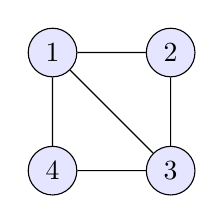
\begin{tikzpicture}[every node/.style={circle,fill=blue!10,draw,minimum size=0.5cm,node distance=1.5cm}]
\node (1) {$1$};
\node[right of=1] (2) {$2$};
\node[below of=2] (3) {$3$};
\node[left of=3] (4) {$4$};
\path[draw] (1) -- (2) -- (3) -- (4) -- (1) -- (3);
\end{tikzpicture}
\end{center}
\end{example}
\end{tcolorbox}

Graf si reprezentujeme jako množinu vrcholů a množinu hran, kde každá hrana je dvojice vrcholů. Lépe se nám bude pracovat s uspořádanými dvojicemi, zvolíme tedy (libovolnou) orientaci hran.
\[
\structure G = \langle V; E \rangle = \langle \{1,2,3,4\}; \{(1,2),(1,3),(1,4),(2,3),(3,4)\} \rangle
\]



Začneme opět formalizací ve výrokové logice. Označme si množinu barev jako \( C=\{R,G,B\} \).  Přirozená volba výrokových proměnných je ``vrchol \(v\) má barvu \(c\)'', označme \(p_v^c\), pro každý vrchol \(v \in V\) a každou barvu \(c\in C\). Naše (uspořádaná) množina výrokových proměnných má 12 prvků:
\[
\mathbb P=\{p_v^c\mid c\in C,v\in V\}=\{p_1^R,p_1^G,p_1^B,p_2^R,p_2^G,p_2^B,p_3^R,p_3^G,p_3^B,p_4^R,p_4^G,p_4^B\}
\]
Máme celkem \( |\M_\mathbb P|=2^{12}=4096 \) modelů jazyka (reprezentovaných 12-dimenzionálními 0--1 vektory). Většinu z nich nelze interpretovat jako obarvení grafu. Například \( v=(1,1,0,0,\dots,0) \) říká, že vrchol 1 je obarvený červeně, a také zeleně. Začneme tedy teorií vyjadřující, že každý vrchol má nejvýše jednu barvu. Existuje více způsobů, jak to můžeme vyjádřit. My řekneme pro každý vrchol, že nesmí mít (alespoň) jednu z každé dvojice barev. Tím dostaneme teorii v {CNF}:

\begin{align*}
T_1 = \{ 
&(\neg p_1^R \lor \neg p_1^G) \land (\neg p_1^R \lor \neg p_1^B) \land (\neg p_1^G \lor \neg p_1^B),\\
&(\neg p_2^R \lor \neg p_2^G) \land (\neg p_2^R \lor \neg p_2^B) \land (\neg p_2^G \lor \neg p_2^B),\\
&(\neg p_3^R \lor \neg p_3^G) \land (\neg p_3^R \lor \neg p_3^B) \land (\neg p_3^G \lor \neg p_3^B),\\
&(\neg p_4^R \lor \neg p_4^G) \land (\neg p_4^R \lor \neg p_4^B) \land (\neg p_4^G \lor \neg p_4^B)\} \\
    = \{ &(\neg p_v^R \lor \neg p_v^G) \land (\neg p_v^R \lor \neg p_v^B) \land (\neg p_v^G \lor \neg p_v^B) \mid v \in V \} 
\end{align*}
Teorii \(T_1\) bychom mohli říkat teorie částečných vrcholových obarvení grafu \(\structure G\). Teorie \(T_1\) má \(|\M_\mathbb P(T_1)|= 4^4=2^8=256\) modelů. (Proč?) Pokud chceme úplná obarvení, přidáme podmínku, že každý vrchol má alespoň jednu barvu.\footnote{Symbol \(\bigvee \) používáme podobně jako symboly \(\sum \) pro součet a \(\prod \) pro součin: ke zjednodušení zápisu výroku, který je ve formě disjunkce. Např.\ pokud \(v=1\), potom \( \bigvee_{c\in C} p_v^c \) reprezentuje výrok \( p_1^R \lor p_1^G \lor p_1^B \). Analogicky \(\bigwedge \) pro konjunkci.}

\begin{align*}
T_2 &= T_1\cup \{p_1^R \lor p_1^G \lor p_1^B, p_2^R \lor p_2^G \lor p_2^B, p_3^R \lor p_3^G \lor p_3^B, p_4^R \lor p_4^G \lor p_4^B\} \\
    &= T_1\cup \{ p_v^R \lor p_v^G \lor p_v^B \mid v \in V \} \\
    &= T_1\cup \{\bigvee_{c\in C} p_v^c \mid v \in V \}  
\end{align*}

Teorie \( T_2 \) má \(3^4=81\) modelů. Jde o \emph{extenzi} teorie \( T_1 \), neboť každý důsledek teorie \( T_1 \) platí i v teorii \( T_2 \). Platí dokonce, že \( \M_\mathbb P(T_2)\subseteq\M_\mathbb P(T_1) \).\footnote{Zde vidíme typickou ukázku antimonotónního vztahu tzv.\ Galoisovy korespondence: čím více vlastností (výroků) požadujeme, tím méně objektů (modelů) splňuje tyto vlastnosti.} Zbývá přidat podmínku zakazující monochromatické hrany. Pro každou hranu a každou barvu specifikujeme, že alespoň jeden z vrcholů hrany nesmí mít danou barvu. Zde pro názornost naposledy napíšeme úplný seznam výroků, nadále budeme využívat zkráceného zápisu.
\begin{align*}
    T_3 = T_2\cup \{ & (\neg p_1^R \lor \neg p_2^R) \land (\neg p_1^G \lor \neg p_2^G) \land (\neg p_1^B \lor \neg p_2^B),\\
    & (\neg p_1^R \lor \neg p_3^R) \land (\neg p_1^G \lor \neg p_3^G) \land (\neg p_1^B \lor \neg p_3^B),\\
    & (\neg p_1^R \lor \neg p_4^R) \land (\neg p_1^G \lor \neg p_4^G) \land (\neg p_1^B \lor \neg p_4^B),\\
    & (\neg p_2^R \lor \neg p_3^R) \land (\neg p_2^G \lor \neg p_3^G) \land (\neg p_2^B \lor \neg p_3^B),\\
    & (\neg p_3^R \lor \neg p_4^R) \land (\neg p_3^G \lor \neg p_4^G) \land (\neg p_3^B \lor \neg p_4^B)\} \\  
= T_2\cup \{ &\bigwedge_{c\in C} 
(\neg p_u^c \lor \neg p_v^c) \mid (u,v) \in E \}
\end{align*}
Výsledná teorie \( T_3 \) je \emph{splnitelná} (má model), právě když graf \( \structure{G} \) je 3-obarvitelný. Má 6 modelů jednoznačně odpovídajících 3-obarvení grafu \( \structure G \). Model \( v = (1,0,0,0,1,0,0,0,1,0,1,0) \) odpovídá následujícímu obarvení, ostatní obarvení získáme permutací barev.
\begin{center}
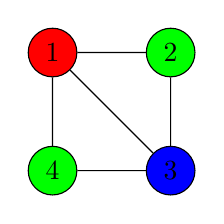
\begin{tikzpicture}[every node/.style={circle,fill=blue!10,draw,minimum size=0.5cm,node distance=1.5cm}]
\node[fill=red] (1) {$1$};
\node[fill=green,right of=1] (2) {$2$};
\node[fill=blue,below of=2] (3) {$3$};
\node[fill=green,left of=3] (4) {$4$};
\path[draw] (1) -- (2) -- (3) -- (4) -- (1) -- (3);
\end{tikzpicture}
\end{center}

Jakmile máme teorii \(T_3\) formalizující 3-obarvení grafu \( \structure{G} \), můžeme snadno řešit související otázky, například najít všechna obarvení, ve kterých je vrchol 1 modrý a vrchol 2 zelený: odpovídají modelům teorie \( T_3 \cup \{ p_1^B, p_2^G\} \). Nebo můžeme dokázat, že vrcholy 2 a 4 musejí být obarveny stejnou barvou. Můžeme použít tablo metodu: v kořeni tabla bude předpoklad
\[
\text{False  }(p_2^R \land p_4^R)\lor(p_2^G \land p_4^G)\lor(p_2^B \land p_4^B)
\]
Nebo můžeme najít rezoluční zamítnutí teorie vzniklé převedením axiomů teorie \( T_3 \) do CNF, a přidáním CNF ekvivalentu \emph{negace} výroku \( (p_2^R \land p_4^R)\lor(p_2^G \land p_4^G)\lor(p_2^B \land p_4^B) \)	(neboť jde o důkaz sporem, tedy pro spor předpokládáme, že \emph{nemají} stejnou barvu).



\section{Predikátová logika}

Nyní si velmi stručně a neformálně představíme \emph{predikátovou logiku}. Predikátová logika se zabývá vlastnostmi objektů a vztahy mezi objekty. Například:
\begin{quote}\it
    Všichni lidé jsou smrtelní.\\
    Sókratés je člověk.\\
    Sókratés je smrtelný.
\end{quote}
Ve skutečnosti výroková logika vznikla později (asi o století) než Aristotelova predikátová logika, a byla poté na dlouho převážně zapomenuta.


\subsection{Nevýhody formalizace ve výrokové logice}\label{subsection:disadvantages-of-propositional-logic}

Nevýhodou formalizace našeho problému ve výrokové logice je fakt, že výsledná teorie \( T_3 \) je poměrně velká, a navíc byla vytvořena ad hoc pro graf  \( \structure{G} \). Představme si, že potřebujeme graf \( \structure{G} \) změnit, například přidáním vrcholu 5 spojeného hranami s vrcholy 2 a 3:

\begin{center}
    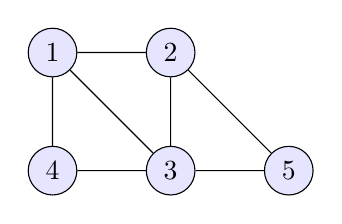
\begin{tikzpicture}[every node/.style={circle,fill=blue!10,draw,minimum size=0.5cm,node distance=1.5cm}]
    \node (1) {$1$};
    \node[right of=1] (2) {$2$};
    \node[below of=2] (3) {$3$};
    \node[left of=3] (4) {$4$};
    \path[draw] (1) -- (2) -- (3) -- (4) -- (1) -- (3);
    \node[right of=3] (5) {$5$};
    \path[draw] (2) -- (5) -- (3);
    \end{tikzpicture}
\end{center}

Abychom byli schopni formalizovat nový problém, musíme přidat do našeho jazyka tři nové výrokové proměnné: \(\mathbb P'=\mathbb P \cup \{ p_5^R,p_5^G,p_5^B\} \), a vytvořit nové teorie \( T'_1, T'_2, T'_3 \) přidáním axiomů týkajících se vrcholu 5 a hran \( (2, 5), (3,5) \). Problémem je, že strukturu grafu \( \structure{G} \) a přirozené vlastnosti jako ``z vrcholu \(u\) vede hrana do vrcholu \(v\)'', nebo ``vrchol \(u\) je zelený'' jsme (`natvrdo', `nepřirozeně') zakódovali do 0--1 proměnných. Tento nedostatek odstraňuje \emph{predikátová logika}.

\subsection{Stručné představení predikátové logiky}

\emph{Modelem} v predikátové logice není 0--1 vektor, ale \emph{struktura}. Příkladem struktur jsou naše (orientované) grafy:
\begin{align*}
    &\structure G = \langle V^\structure G; E^\structure G \rangle = \langle \{1,2,3,4\}; \{(1,2),(1,3),(1,4),(2,3),(3,4)\} \rangle \\ 
    &\structure{G}' = \langle V^{\structure{G}'}; E^{\structure{G}'} \rangle = \langle \{1,2,3,4,5\}; \{(1,2),(1,3),(1,4),(2,3),(3,4),(2,5),(3,5)\} \rangle
\end{align*}
Oba grafy sestávají z množiny vrcholů, a z binární relace na této množině. Jde o struktury v \emph{jazyce teorie grafů} \( \mathcal L=\langle E \rangle \), kde \(E\) je binární \emph{relační symbol}. \emph{Jazyk} predikátové logiky specifikuje jaké relace (kolik a jakých arit --- unární, binární, ternární, atd.) mají struktury mít, a jaké symboly pro ně budeme používat. Kromě toho používáme symbol rovnosti \(=\) a struktury mohou obsahovat také funkce a konstanty (jako například funkce \( +,-,\cdot \) a konstanty $0,1$ v \emph{tělese} reálných čísel), ty si ale necháme na později.

Predikátová logika používá tytéž logické spojky jako výroková logika, ale základním stavebním kamenem \emph{predikátových formulí} nejsou výrokové proměnné, nýbrž tzv.\ \emph{atomické formule}, například: \( E(x,y) \) představuje tvrzení, že v grafu vede hrana z vrcholu \(x\) do vrcholu \(y\). Zde \(x,y\) jsou \emph{proměnné} reprezentující vrcholy daného grafu. Kromě toho ve formulích můžeme používat \emph{kvantifikátory}: \( (\forall x) \) ``pro všechny vrcholy \(x\)'' a \( (\exists y) \) ``existuje vrchol \(y\)''.\footnote{Kvantifikátory si můžeme představit jako ``konjunkci'' resp.\ ``disjunkci'' přes všechny vrcholy grafu.} 

Nyní můžeme formalizovat tvrzení, která dávají smysl pro libovolný graf. Například: 
\begin{itemize}
    \item ``V grafu nejsou smyčky'': \[ (\forall x)(\neg E(x,x)) \] 
    \item ``Existuje vrchol výstupního stupně 1'': \[ (\exists x)(\exists y)(E(x,y) \land (\forall z)(E(x,z) \limplies y=z)) \] 
\end{itemize}
V daném grafu \(\structure{G}\) a při dosazení vrcholu \(u\) za proměnnou \(x\) a vrcholu \(v\) za proměnnou \(y\) vyhodnotíme \( E(x,y) \) jako True, právě když \( (u,v)\in E^{\structure{G}} \).


\subsection{Formalizace barvení grafů v predikátové logice}


Vraťme se zpět k barvení grafů. Přirozený způsob jak formalizovat náš problém 3-obarvitelnosti je v jazyce \( \mathcal L' =\langle E, R, G, B \rangle \), kde \(E\) je binární a \(R,G,B\) jsou unární relační symboly, tedy \(R(x)\) znamená ``vrchol \(x\) je červený''. Strukturou pro tento jazyk je (orientovaný) graf spolu s trojicí množin vrcholů, např.
\begin{align*}
\structure G_C &= \langle V^{\structure G_C}; E^{\structure G_C}, R^{\structure G_C}, G^{\structure G_C}, B^{\structure G_C} \rangle \\
&= \langle \{1,2,3,4\}; \{(1,2),(1,3),(1,4),(2,3),(3,4)\}, \{1\}, \{2,4\}, \{3\} \rangle    
\end{align*}
reprezentuje graf \( \structure{G} \) s validním obarvením z obrázku výše. Budeme říkat, že \( \structure{G}_C \) je \emph{expanze} \(\mathcal L\)-struktury \( \structure{G} \) do jazyka \( \mathcal L' \).

Podobně jako ve výrokové logice musíme nejprve zajistit, aby naše modely reprezentovaly obarvené grafy. Začneme požadavkem, aby každý vrchol byl obarven nejvýše jednou barvou:
\[
(\forall x)((\neg R(x) \lor \neg G(x)) \land (\neg R(x) \lor \neg B(x)) \land (\neg G(x) \lor \neg B(x)))
\]
Obarvení alespoň jednou barvou vyjádříme takto:
\[
(\forall x)(R(x) \lor G(x) \lor B(x))
\]
A hranovou podmínku formalizujeme pomocí predikátu \( E(x,y) \) například takto:
\[	
(\forall x)(\forall y)(E(x,y) \limplies ((\neg R(x) \lor \neg R(y)) \land (\neg G(x) \lor \neg G(y)) \land (\neg B(x) \lor \neg B(y))))
\]
Modely takto vzniklé teorie reprezentují orientované grafy s vrcholovým 3-obarvením. 


\section{Další druhy logických systémů}

Predikátové logice, kde proměnné reprezentují jednotlivé vrcholy, říkáme logika \emph{prvního řádu} (anglicky  \emph{first-order (FO) logic}). V logice \emph{druhého řádu} (anglicky \emph{second-order (SO) logic}) máme také proměnné reprezentující množiny vrcholů nebo i množiny \(n\)-tic vrcholů (tj.\ relace, funkce). Například tvrzení, že daný graf je bipartitní, můžeme formalizovat v logice druhého řádu následující formulí, ve které $S$ je \emph{proměnná druhého řádu} reprezentující množinu vrcholů a $S(x)$ vyjadřuje, že ``vrchol $x$ je prvkem množiny $S$'':
$$
(\exists S)(\forall x)(\forall y)(E(x,y)\limplies (S(x)\liff\neg S(y)))
$$
Jako jiný, důležitý příklad uveďme tvrzení, že každá neprázdná zdola omezená podmnožina má infimum,\footnote{Což platí v uspořádané množině reálných čísel, ale neplatí v racionálních číslech, např.\ \( \{x \mid x^2 > 2, x > 0\} \).} které můžeme formalizovat v logice druhého řádu takto:\footnote{I když je tato formule velmi složitá, pokuste se porozumět jednotlivým částem.}
\begin{align*}
&(\forall S)((\exists x)S(x) \land (\exists x)(\forall y)(S(y) \limplies x\leq y) \limplies  {}\\ 
&(\exists x)((\forall y)(S(y) \limplies x\leq y) \land (\forall z)((\forall y)(S(y) \limplies z\leq y)\limplies z\leq x)))
\end{align*}
A v logice \emph{třetího řádu} máme i proměnné reprezentující množiny množin (což je užitečné např.\ v topologii), atd.

Kromě výrokové a predikátové logiky existují i další typy logických systémů, například intuicionistická logika (která povoluje jen konstruktivní důkazy), temporální logiky (kde mluvíme o platnosti `vždy', `někdy v budoucnosti', `dokud' apod.), modální logiky (`je možné', `je nutné'), nebo fuzzy logiky (kde máme výroky `0.35 pravdivé'). Tyto logiky mají důležité aplikace v informatice, např.\ v umělé inteligenci (modální logiky pro uvažování autonomních agentů o svém okolí), v paralelním programování (temporální logiky), nebo v automatických pračkách (fuzzy logiky). %Více viz Příloha~\ref{appendix:other-logics}. 
V tomto kurzu se omezíme na výrokovou logiku a predikátovou logiku prvního řádu.


\section{O přednášce}

Přednáška je rozdělena na tři části: 

První část se zabývá výrokovou logikou. Nejprve představíme syntaxi a sémantiku, dále problém splnitelnosti CNF formulí (známý NP-úplný problém SAT) a jeho polynomiálně řešitelné fragmenty (2-SAT, Horn-SAT). Ukážeme si také použití SAT solveru v praxi. Budeme pokračovat tablo metodu, u níž si dokážeme korektnost a úplnost, a také několik aplikací, například Větu u kompaktnosti. A na závěr představíme rezoluční metodu ve výrokové logice.

Ve druhé části představíme predikátovou logiku. Začneme opět syntaxí a sémantikou, ukážeme si jak lze adaptovat tablo metodu pro predikátovou logiku, a skončíme znovu rezoluční metodou. Kromě toho zmíníme několik praktických aplikací, např. databázové dotazy a logické programování (jazyk Prolog). Struktura výkladu v této části je silně provázaná s předchozí částí. Řada definic, vět, důkazů, i algoritmů bude velmi podobná svým protějškům ve výrokové logice. Lišit se budou převážně jen na nízké úrovni, v technických vnitřnostech. Proto je důležité dobře si uspořádat chápání výrokové logiky, než se pustíme do logiky predikátové. 

Třetí, rozsahem nejmenší část je úvodem do teorie modelů, definovatelnosti, axiomatizovatelnosti, a algoritmické rozhodnutelnosti. Jde o ochutnávku pokročilejších témat, která potkáte spíše v teoretické informatice a matematické logice, byť některá mají své místo i v informatice aplikované. Na závěr si představíme slavné Gödelovy věty o neúplnosti, které ukazují meze formální metody (formální dokazatelnosti v axiomatickém systému). 

